\documentclass[10pt,a4paper]{article}
\usepackage[margin=1.0in]{geometry}
\usepackage[utf8]{inputenc}
\usepackage{amsmath}
\usepackage{amsfonts}
\usepackage{amssymb}

\usepackage{graphicx}

\title{Partitioned Element Methods for Non-linear Computational Solid Mechanics}
\author{B. D. Giffin}
\date{\today}

\begin{document}
\maketitle

\abstract{A generalized computational framework for a class of polytopal finite element methods is proposed, leveraging a geometric partitioning of the element domain for the sake of establishing a consistent quadrature scheme. Conventional polytopal element methods either seek to define a set of finite element shape functions explicitly, or implicitly. In the former case, the resulting shape functions are generally non-polynomial in form, leading to inconsistencies in the resulting integration of weak form integrals. In the latter case, only the low-order deformation response of the element can be integrated (via effective mean quadrature over the entire element), necessitating the introduction of artificial stabilization. In the present approach, shape functions are defined in an approximate sense over the element partition to help facilitate integration consistency and stability.}

\section{Introduction}

\section{Weak approximations to the element shape functions}

\subsection{Cells}

Consider a polyhedral element $\Omega$ which has been partitioned into a collection of polyhedral cells $\omega \subset \Omega$, and suppose that each cell is bounded by a collection of polygonal facets $\sigma \subset \partial \omega$. Let the value of a given function $u$ be defined independently on the boundary of each cell and its interior, such that
\begin{equation}
  u = \left\{ \begin{array}{cc} u |_{\omega} & \forall \mathbf{X} \in \omega \\ u |_{\sigma} & \forall \mathbf{X} \in \sigma \subset \partial \omega \end{array} \right. ,
\end{equation}
where the trace of $u |_{\omega}$ evaluated on $\sigma$ is not necessarily the same as $u |_{\sigma} \, \forall \sigma \subset \partial \omega$.
The weak gradient $\nabla_w u |_{\omega} \in \mathcal{V} (\omega)$ of $u$ defined on $\omega$ satisfies the following variational equality:
\begin{equation}
  \int_{\omega} \nabla_w u |_{\omega} \cdot \mathbf{v} \, dV = - \int_{\omega} u |_{\omega} (\nabla \cdot \mathbf{v}) \, dV + \sum_{\sigma \subset \partial \omega} \int_{\sigma} u |_{\sigma} \, \mathbf{v} \cdot d\mathbf{A} |_\sigma \qquad \forall \mathbf{v} \in \mathcal{V} (\omega),
\end{equation}
weakly relating the values on the boundary and interior of the cell.

In a low-order approximation, let it be assumed that the weak gradient $\nabla_{w} u |_{\omega} \in \mathbb{R}^3$ is defined to be constant over $\omega$, such that
\begin{equation}
  \nabla_{w} u |_{\omega} = \frac{1}{|\omega|} \sum_{\sigma \subset \partial \omega} \int_{\sigma} u |_{\sigma} \, d\mathbf{A} |_\sigma,
\end{equation}
and the cell volume $|\omega| \equiv \int_{\omega} dV$ may be equivalently computed from an integral over $\partial \omega$:
\begin{equation}
  |\omega| = \frac{1}{3} \sum_{\sigma \subset \partial \omega} \int_{\sigma} \mathbf{X} \cdot d\mathbf{A} |_\sigma.
\end{equation}
Moreover, let $u |_{\omega} \in \mathbb{R}$ be assumed constant over $\omega$, such that
\begin{equation}
	u |_{\omega} = \frac{1}{3} \left[ \frac{1}{| \omega |} \sum_{\sigma \subset \partial \omega} \int_{\sigma} u |_{\sigma} \, \mathbf{X} \cdot d\mathbf{A} |_\sigma - \bar{\mathbf{X}} |_{\omega} \cdot \nabla_{w} u |_{\omega} \right],
\end{equation}
and the cell centroid $\bar{\mathbf{X}} |_{\omega} = \frac{1}{|\omega|} \int_{\omega} \mathbf{X} \, dV$ may be equivalently computed via
\begin{equation}
	 \bar{\mathbf{X}} |_{\omega} = \frac{1}{4 | \omega |} \sum_{\sigma \subset \partial \omega} \int_{\sigma} (\mathbf{X} \otimes \mathbf{X}) \cdot d\mathbf{A} |_\sigma .
\end{equation}
Consequently, both the average value and (weak) gradient of $u$ are explicitly defined (via linear operators) in terms of the boundary values $u |_{\sigma} \, \forall \sigma \subset \partial \omega$. Moreover, these relations establish local integration consistency over each cell $\omega$, which by extension guarantees integration consistency over the element $\Omega$ as a whole, assuming that any boundary integrals over the exterior of the element are carried out sufficiently accurately, given a particular choice for the discrete representations of $u |_{\sigma}$.

\subsection{Facets}

\begin{figure} [!ht]
	\centering
	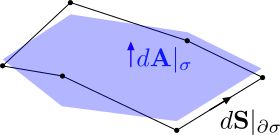
\includegraphics[width = 3.0in]{figures/facet.pdf}
	\caption{A representative polygonal facet.}
	\label{fig:facet}
\end{figure}

Consider a planar polygonal facet $\sigma$ with unit normal $\mathbf{N} |_{\sigma}$ whose boundary consists of a collection of co-planar segments $\bar{\gamma} \subset \partial \sigma$ with their unit tangent vectors denoted $\boldsymbol{\lambda} |_{\bar{\gamma}}$. Let each segment $\bar{\gamma}$ be the planar projection of a corresponding segment $\gamma$ (refer to figure \ref{fig:facet}.) The projected segments are defined via the differential transform $d \mathbf{S} |_{\bar{\gamma}} = \mathbf{P} |_{\sigma} \cdot d \mathbf{S} |_{\gamma}$, where $\mathbf{P} |_{\sigma} = \mathbf{1} - \mathbf{N} |_{\sigma} \otimes \mathbf{N} |_{\sigma}$ constitutes a planar projection operator for the facet $\sigma$, $d \mathbf{S} |_{\gamma} = \boldsymbol{\lambda} |_{\gamma} \, dS |_{\gamma}$ is the directed differential length of the segment $\gamma$, and $d \mathbf{S} |_{\bar{\gamma}} = \boldsymbol{\lambda} |_{\bar{\gamma}} \, dS |_{\bar{\gamma}}$ is its corresponding projection onto the plane containing $\sigma$.
Additionally, let $d \mathbf{N} |_{\bar{\gamma}} = d \mathbf{S} |_{\gamma} \times \mathbf{N} |_{\sigma}$ be the differential length times the projected outward normal to the boundary of $\sigma$.

Recursively, let it be supposed that the scalar field $u$ is defined independently on each polygonal facet $\sigma$ and its bounding segments $\gamma \subset \partial \sigma$, such that
\begin{equation}
  u = \left\{ \begin{array}{cc} u |_{\sigma} & \forall \mathbf{X} \in \sigma \\ u |_{\gamma} & \forall \mathbf{X} \in \gamma \subset \partial \sigma \end{array} \right. ,
\end{equation}
where again, the trace of $u |_{\sigma}$ evaluated on $\bar{\gamma}$ is not necessarily the same as $u |_{\gamma} \forall \gamma \subset \partial \sigma$.

Using the definition of the weak gradient defined on $\sigma$:
\begin{equation}
  \int_{\sigma} \nabla_w u |_{\sigma} \cdot \mathbf{v} \, dA = - \int_{\sigma} u |_{\sigma} (\nabla \cdot \mathbf{v}) \, dA + \sum_{\gamma \subset \partial \sigma} \int_{\gamma} u |_{\gamma} \, \mathbf{v} \times d \mathbf{S} |_{\gamma} \cdot \mathbf{N} |_{\sigma} \qquad \forall \mathbf{v} \in \mathcal{V} (\sigma),
\end{equation}
the area of the facet $| \sigma | \equiv \int_\sigma \, dA$ may therefore be computed via
\begin{equation}
	| \sigma | = \frac{1}{2} \sum_{\gamma \subset \partial \sigma} \int_{\gamma} \mathbf{X} \times d\mathbf{S} |_{\gamma} \cdot \mathbf{N} |_{\sigma}.
\end{equation}
Up to this point, the precise means by which the facet normal $\mathbf{N} |_{\sigma}$ is determined has been left unspecified. As a particular choice, let $\mathbf{N} |_{\sigma}$ be chosen such that $| \sigma |$ is a maximum, yielding the following definition for the directed discrete differential area $d\mathbf{A} |_{\sigma} = |\sigma| \, \mathbf{N} |_{\sigma}$ of the facet $\sigma$ in terms of a boundary integral over the (non-planar) segmented boundary:
\begin{equation}
	d\mathbf{A} |_{\sigma} \equiv \frac{1}{2} \sum_{\gamma \subset \partial \sigma} \int_{\gamma} \mathbf{X} \times d\mathbf{S} |_{\gamma}.
\end{equation}

Following similar arguments as before, the average value $u |_{\sigma} \in \mathbb{R}$ and weak in-plane gradient $\nabla_w u |_{\sigma} \in \mathbb{R}^3$ defined on $\sigma$ are given by
\begin{equation}
  \nabla_{w} u |_{\sigma} = \frac{1}{|\sigma|} \sum_{\gamma \subset \partial \sigma} \int_{\gamma} u |_{\gamma} \, d\mathbf{S} |_{\gamma} \times \mathbf{N} |_{\sigma},
\end{equation}
where $|\sigma| \equiv \int_{\sigma} dA$, and
\begin{equation}
	u |_{\sigma} = \frac{1}{2} \left[ \frac{1}{| \sigma |} \sum_{\gamma \subset \partial \sigma} \int_{\gamma} u |_{\gamma} \, \mathbf{X} \times d\mathbf{S} |_{\gamma} \cdot \mathbf{N} |_{\sigma} - \bar{\mathbf{X}} |_{\sigma} \cdot \nabla_{w} u |_{\sigma} \right] ,
\end{equation}
where $\bar{\mathbf{X}} |_{\sigma} \equiv \frac{1}{|\sigma|} \int_{\sigma} \mathbf{X} \, dA$ can be evaluated via
\begin{equation}
	\bar{\mathbf{X}} |_{\sigma} = \frac{1}{3 | \sigma |} \sum_{\gamma \subset \partial \sigma} \int_{\gamma} \mathbf{X} |_{\gamma} ( \mathbf{X} \times d\mathbf{S} |_{\gamma} \cdot \mathbf{N} |_{\sigma}) - \mathbf{N} |_{\sigma} \frac{1}{12 | \sigma |} \sum_{\gamma \subset \partial \sigma} \int_{\gamma} (\mathbf{N} |_{\sigma} \cdot \mathbf{X} |_{\gamma}) \, \mathbf{X} \times d\mathbf{S} |_{\gamma} \cdot \mathbf{N} |_{\sigma}.
\end{equation}
It follows that for a given facet $\sigma$ with normal $\mathbf{N}$ defined in the reference configuration of the element (prior to deformation by the mapping $\mathbf{x} = \chi (\mathbf{X},t)$, the transformed surface area element is characterized by Nanson's relation:
\begin{equation}
	\mathbf{n} \, da = \text{cof} \left( \nabla_w \mathbf{x} |_{\sigma} \right) \cdot \mathbf{N} \, dA,
\end{equation}
where the matrix cofactor $\text{cof} \left( \mathbf{A} \right)$ can be safely evaluated for any (possibly rank deficient) $3\times3$ matrix $\mathbf{A}$ via the following formula:
\begin{equation}
	\text{cof} \left( \mathbf{A} \right)_{ij} = \frac{1}{2} \varepsilon_{mni} \varepsilon_{pqj} A_{pm} A_{qn} .
\end{equation}
The above formula should always be used, as $\nabla_w \mathbf{x} |_{\sigma}$ may become indefinite.

\subsection{Segments}

Finally, assume that for each linear segment $\gamma \subset \partial \sigma$ whose endpoints consist of the two vertices $\left\{ v_1, v_2 \right\} = \partial \gamma$, the assumed constant weak gradient $\nabla_w u |_{\gamma}$ and constant average value $u |_{\gamma}$ are given by
\begin{equation}
  \nabla_{w} u |_{\gamma} = \frac{1}{|\gamma|} (u |_{v_2} - u |_{v_1}) \boldsymbol{\lambda} |_{\gamma},
\end{equation}
where $|\gamma| \equiv \int_{\gamma} dS = || \mathbf{X} |_{v_2} - \mathbf{X} |_{v_1} ||_2$, and
\begin{equation}
	u |_{\gamma} = \frac{1}{| \gamma |} (u |_{v_2} \mathbf{X}' |_{v_2} - u |_{v_1} \mathbf{X}' |_{v_1}) \cdot \boldsymbol{\lambda} |_{\gamma},
\end{equation}
where $\mathbf{X}' \equiv \mathbf{X} - \bar{\mathbf{X}}$, $\bar{\mathbf{X}} \equiv \frac{1}{|\gamma|} \int_{\gamma} \mathbf{X} \, dS = \frac{1}{2} (\mathbf{X} |_{v_1} + \mathbf{X} |_{v_2})$, and $\boldsymbol{\lambda} |_{\gamma} = \frac{1}{| \gamma |} (\mathbf{X} |_{v_2} - \mathbf{X} |_{v_1})$.

\section{Integration consistency}



\section{Stability}



\end{document}
